\RequirePackage[l2tabu, orthodox]{nag}
\documentclass[final, unknownkeysallowed]{beamer}
\usetheme{RJH}
\usepackage[orientation=portrait, size=a2, scale=1.4, debug]{beamerposter}
\usepackage{caption}
\usepackage[absolute, overlay]{textpos}
\setlength{\TPHorizModule}{1cm}
\setlength{\TPVertModule}{1cm}

\title{Clinical Science -- Medical Physics and Bioinformatics}
\author{\textbf{Gavin Kirby, PhD --- \textit{gavin.kirby@uhb.nhs.uk}}}
\institute[UHB]{University Hospitals Birmingham NHS Foundation Trust}
\footer{Scientific Computing in Radiotherapy Physics}
\date{2020-01-10}

\begin{document}
\begin{textblock}{6}(1.0, 0.15)
    
\includegraphics[height = 23 mm]{uhb-logo.png}
\end{textblock}
\begin{textblock}{6}(38.0, 0.0)
    
\includegraphics[height = 23 mm]{lgbtstem_test_transparent.png}
\end{textblock}
\begin{frame}{}
%
\begin{textblock}{19.5}(1, 4.5)
    \begin{block}{Clinical science -- use scientific knowledge for tangible benefit}
        \begin{itemize}
            \item Broadly: \textit{applied science for patient benefit}.
            \item Basic r\^{o}le of a clinical scientist comprises:
                \begin{itemize}
                    \item Quality assurance of equipment.
                    \item Auditing to ensure compliance with legislation \& best practice guidelines.
                    \item Translational research \& service development.
                    \item Providing scientific advice to clinical services.
                    \item Teaching \& training of scientists, physicians, and technologists.
                \end{itemize}
        \end{itemize}
    \end{block}
%
    \begin{block}{Clinical radiotherapy physics -- routine work}
        \begin{itemize}
            \item Broad specialism within medical physics.
            \item Radiation dosimetry and treatment planning.
            \item External-beam X-ray and electron therapies, and brachytherapy.
            \item Important intersection with radiology (CT \& MR).
        \end{itemize}
        \begin{figure}
            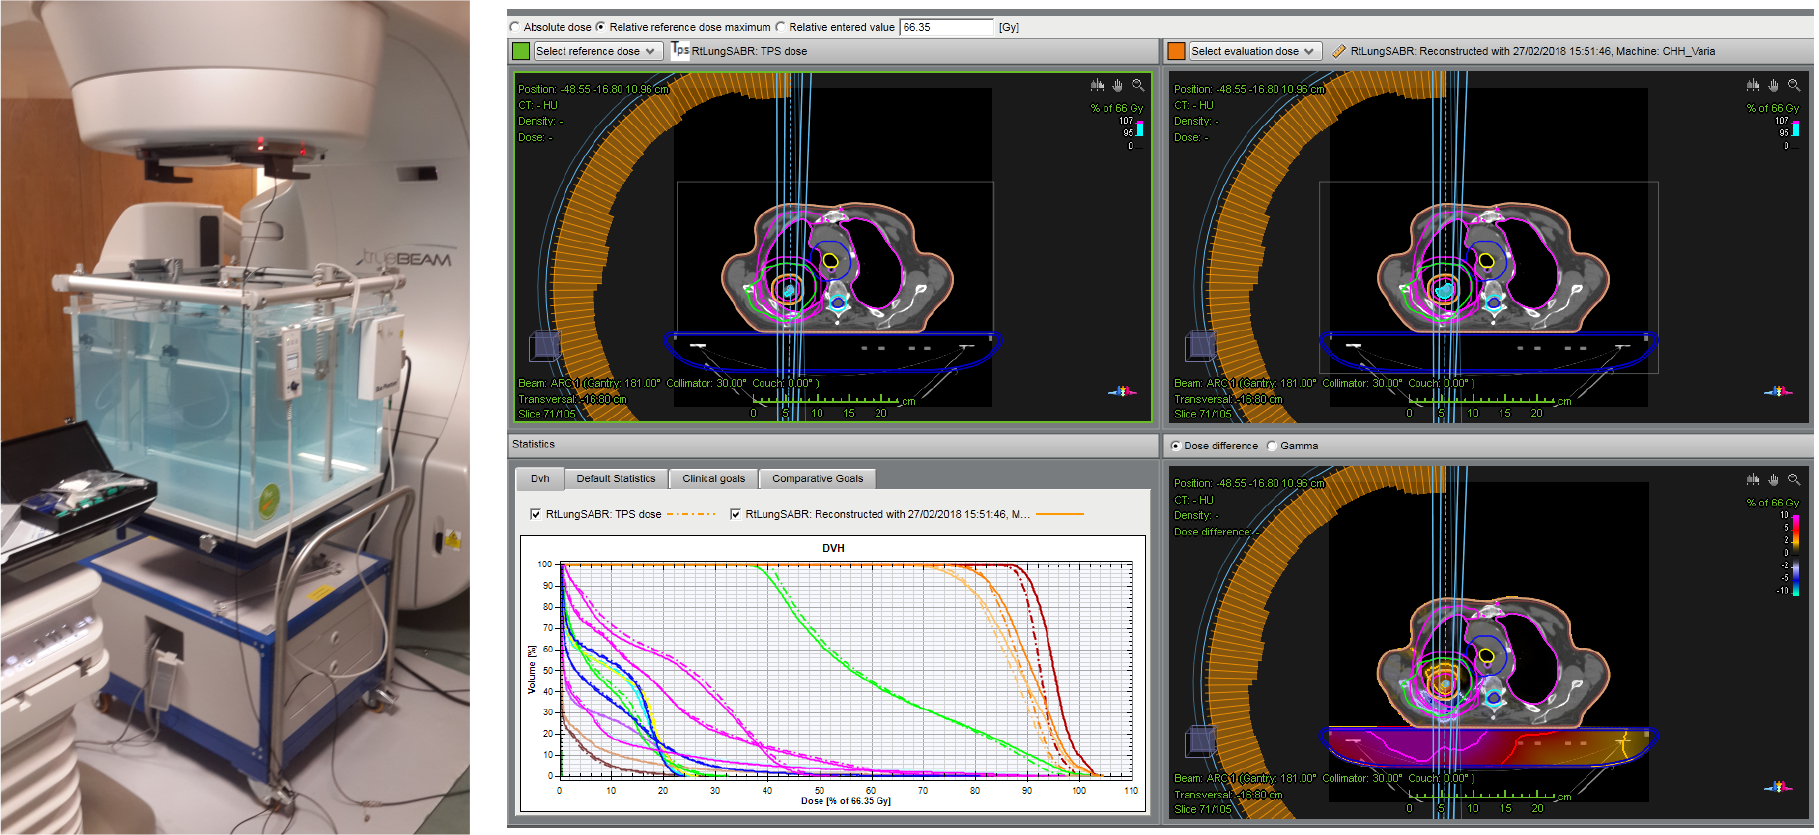
\includegraphics[width = \textwidth]{rt_physics_gamma.png}
            \caption*{Using a water tank phantom for relative dosimetry during linac commissioning (L); a gamma analysis is performed to assess a treatment machine's delivery of a lung treatment plan against the treatment-planning system prediction (R).}\label{fig:watertank}
        \end{figure}
    \end{block}
%
    \begin{block}{Bioinformatics in the physical sciences}
        \begin{itemize}
            \item Broadly: \textit{intersection of scientific computing and life sciences}.
            \item Medical physics depends heavily on computing -- \textit{e.g.} calculation of radiation doses, image quality optimisation, and optimisation of treatment plans.
            \item Computing essential for research and service development -- data analysis and automation of workflow; commissioning of new software.
            \item In-house software development -- bespoke, robust tools to satisfy departmental requirements \& aid in meeting (inter)national guidelines.
        \end{itemize}
    \end{block}
%
    \begin{block}{Putting it together to develop the service}
        \begin{itemize}
            \item Integrate developments in computing into clinical workflow.
            \item Transition to paperless/lite system ${\rightarrow}$ increased efficiency \& safety.
            \item Dashboards for workflow visualisation and easy data exploration -- existing commercial solutions do not provide such bespoke functionality in a single application. Facilitate auditing and service development.
            \item Scripting for treatment planning systems -- automate routine tasks such as organ contouring and beam placement.
        \end{itemize}
    \end{block}

    \begin{block}{Knowledge-based planning: plan evaluation}
        \begin{figure}
          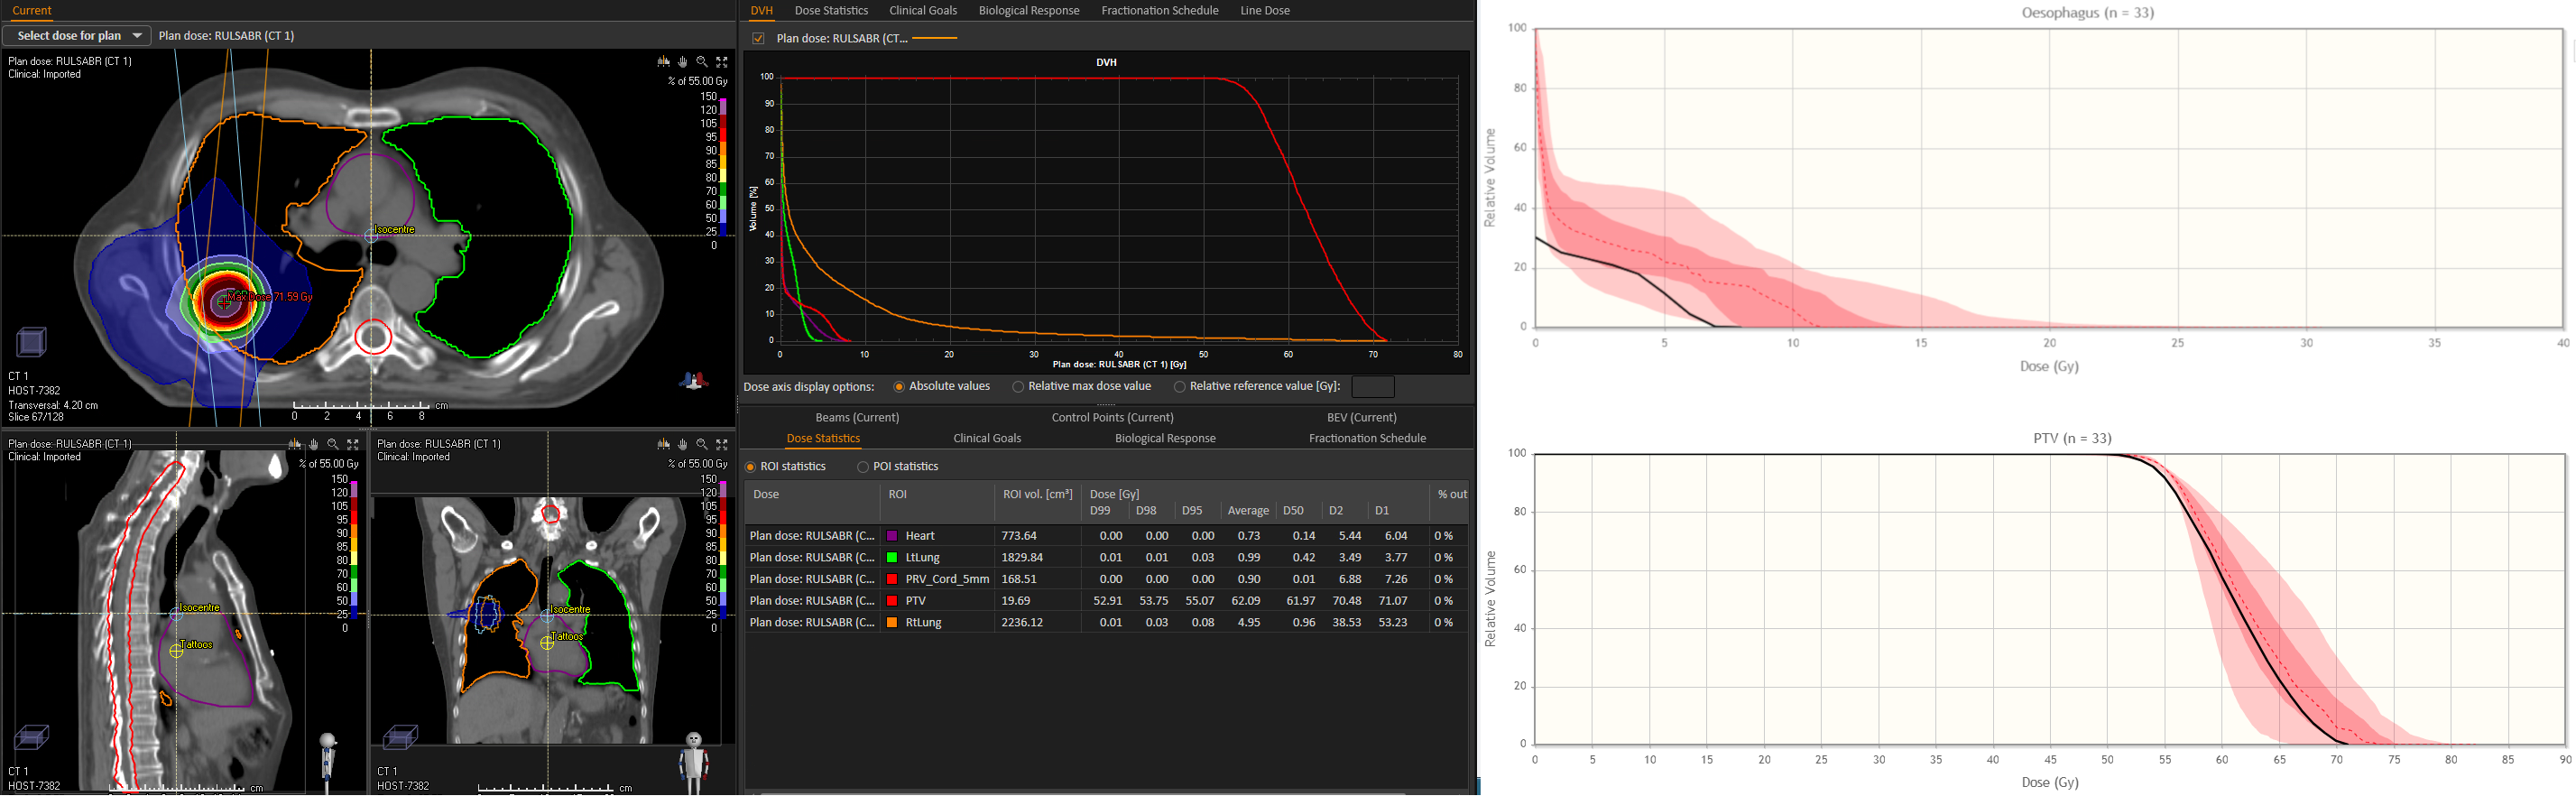
\includegraphics[width = \textwidth]{dvh_analysis.png}
          \caption*{A dashboard application developed by the UHB clinical computing science group for comparison of dose-volume histogram data against a population of historical patients (``good'' plans). Here, a lung plan (in the RayStation treatment planning system, L) is analysed in terms of organ-at-risk sparing (top R) and target coverage (bottom R).}\label{fig:kbp}
        \end{figure}
      \end{block}
\end{textblock}
%
\begin{textblock}{19.3}(21.8, 4.5)
    \begin{block}{QATrack+ -- streamline and automate QA}
        \begin{figure}
          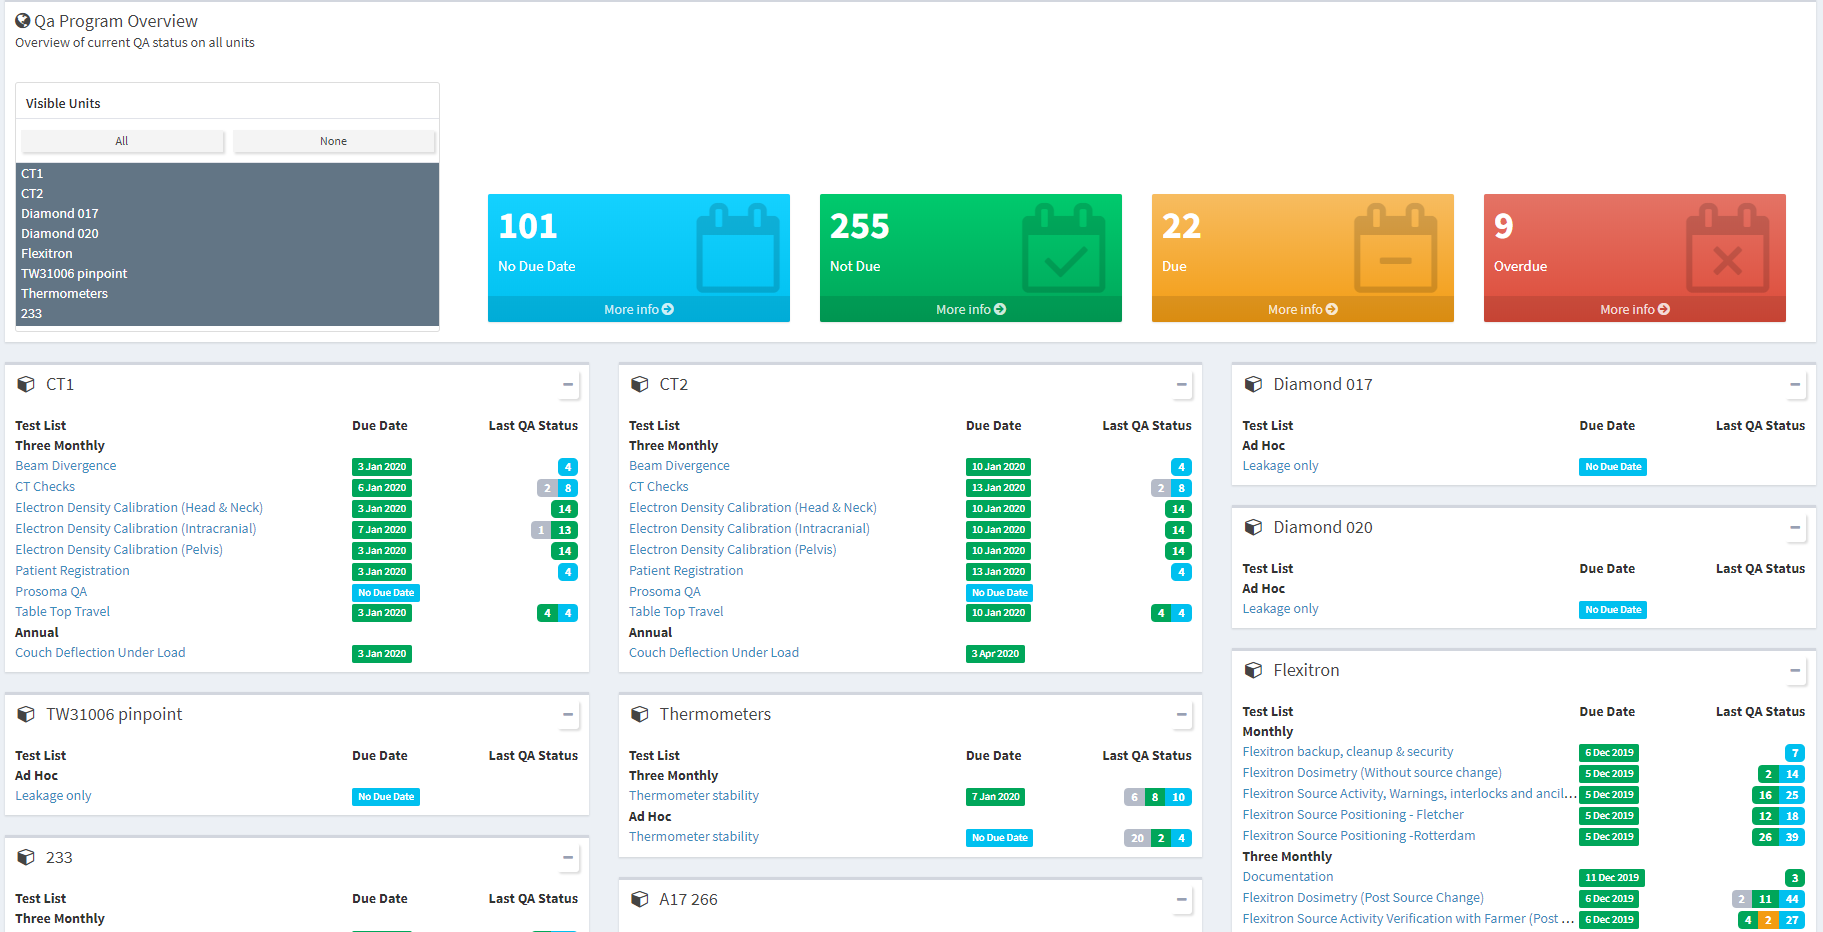
\includegraphics[width = \textwidth]{qatrack_dashboard.png}
%          \caption*{QATrack+ graphical overview dashboard showing the current status of all machines. QATrack+ facilitates the integration, scheduling, recording and analysis of all departmental QA work. Development of QATrack+ involves its commissioning, validation and deployment into routine practice.}
            \caption*{Project to commission QATrack+ and deploy it into routine practice -- this software greatly facilitates the integration, scheduling, recording, and analysis of all departmental QA work. This is its overview dashboard, showing the current status of all machines.}\label{fig:qatrack_dashboard}
        \end{figure}
        \begin{figure}
            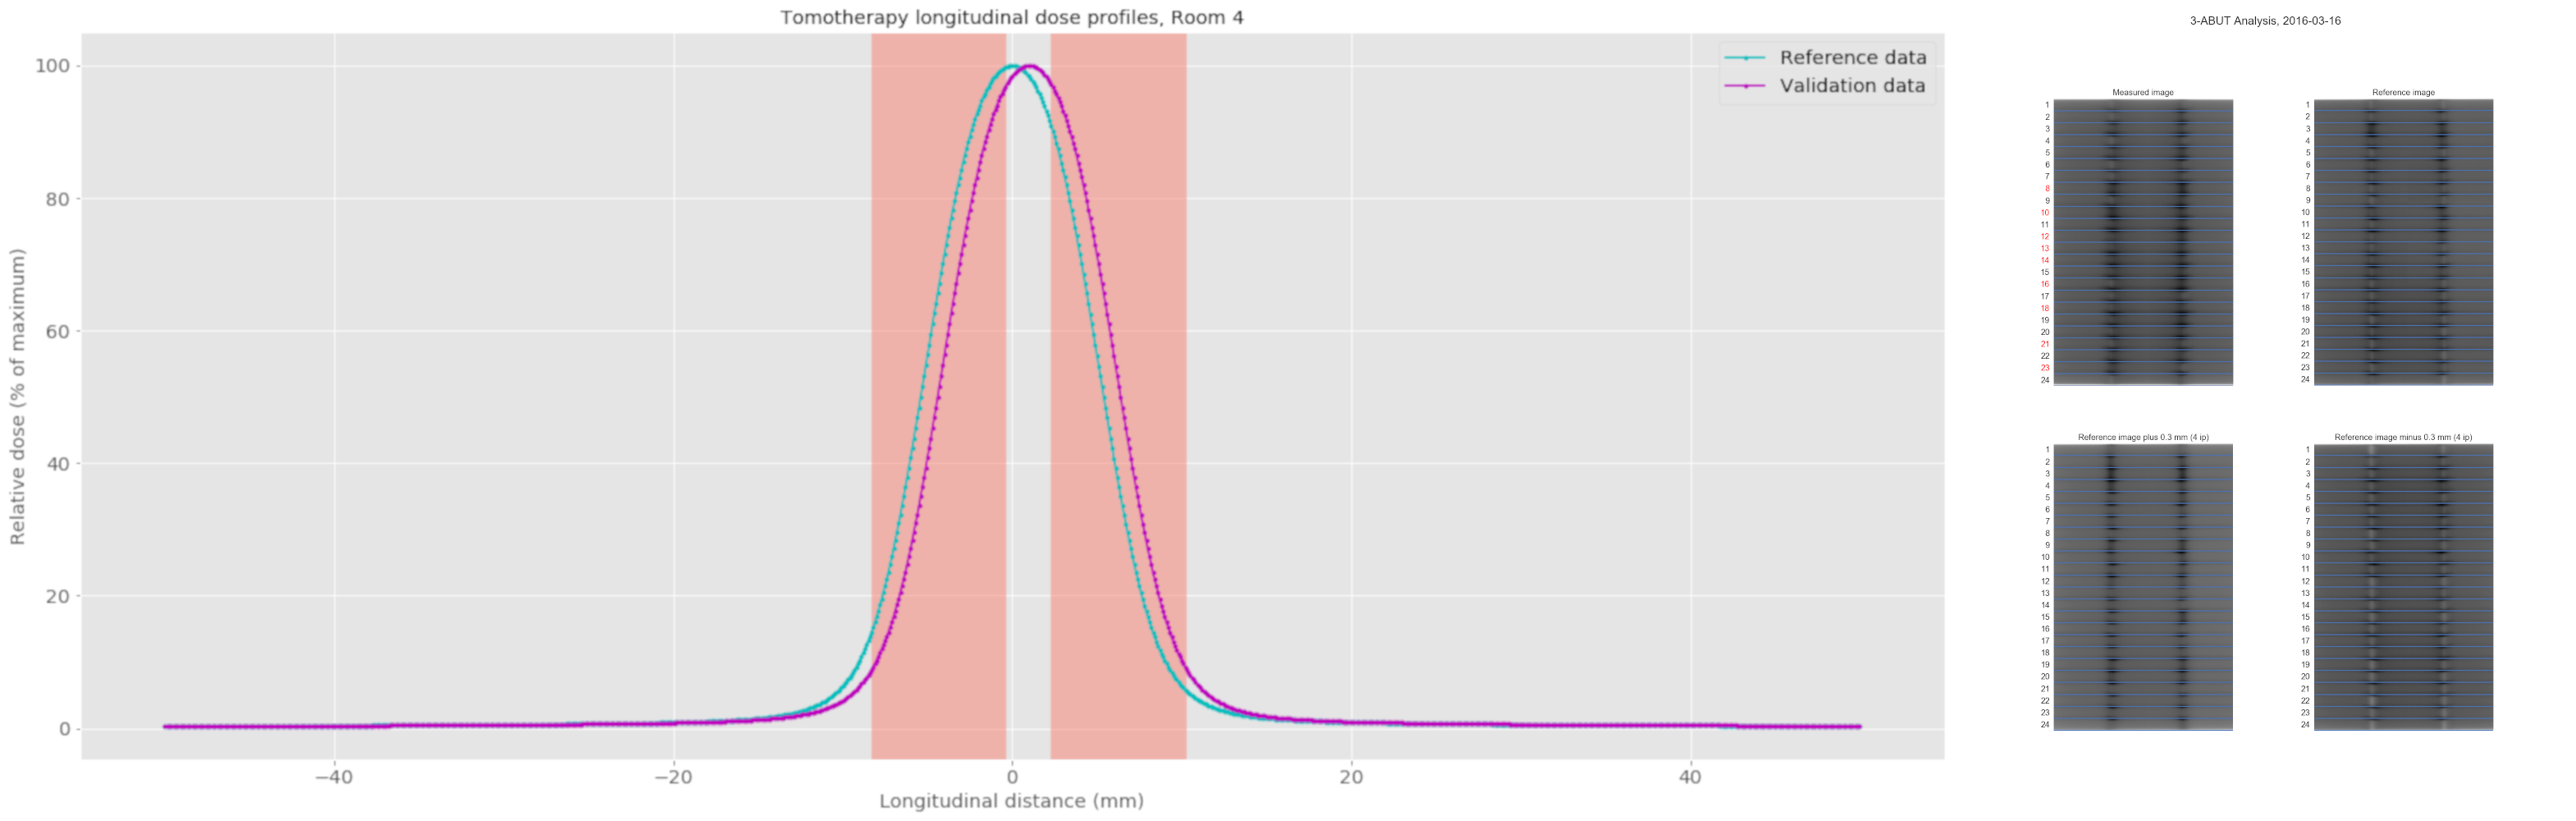
\includegraphics[width = \textwidth]{qatrack_analysis.png}
            \caption*{Automated QA -- comparison of a measured photon beam profile against expected (L) and assessment of multileaf collimator leaf positions against their respective tolerances (3-abut analysis, R). Increased automation allows physicists to focus on non-routine work.}\label{fig:qatrack_analysis}
        \end{figure}
    \end{block}
%
    \begin{block}{Research -- CyberKnife patient respiratory motion analysis}
        \begin{figure}
            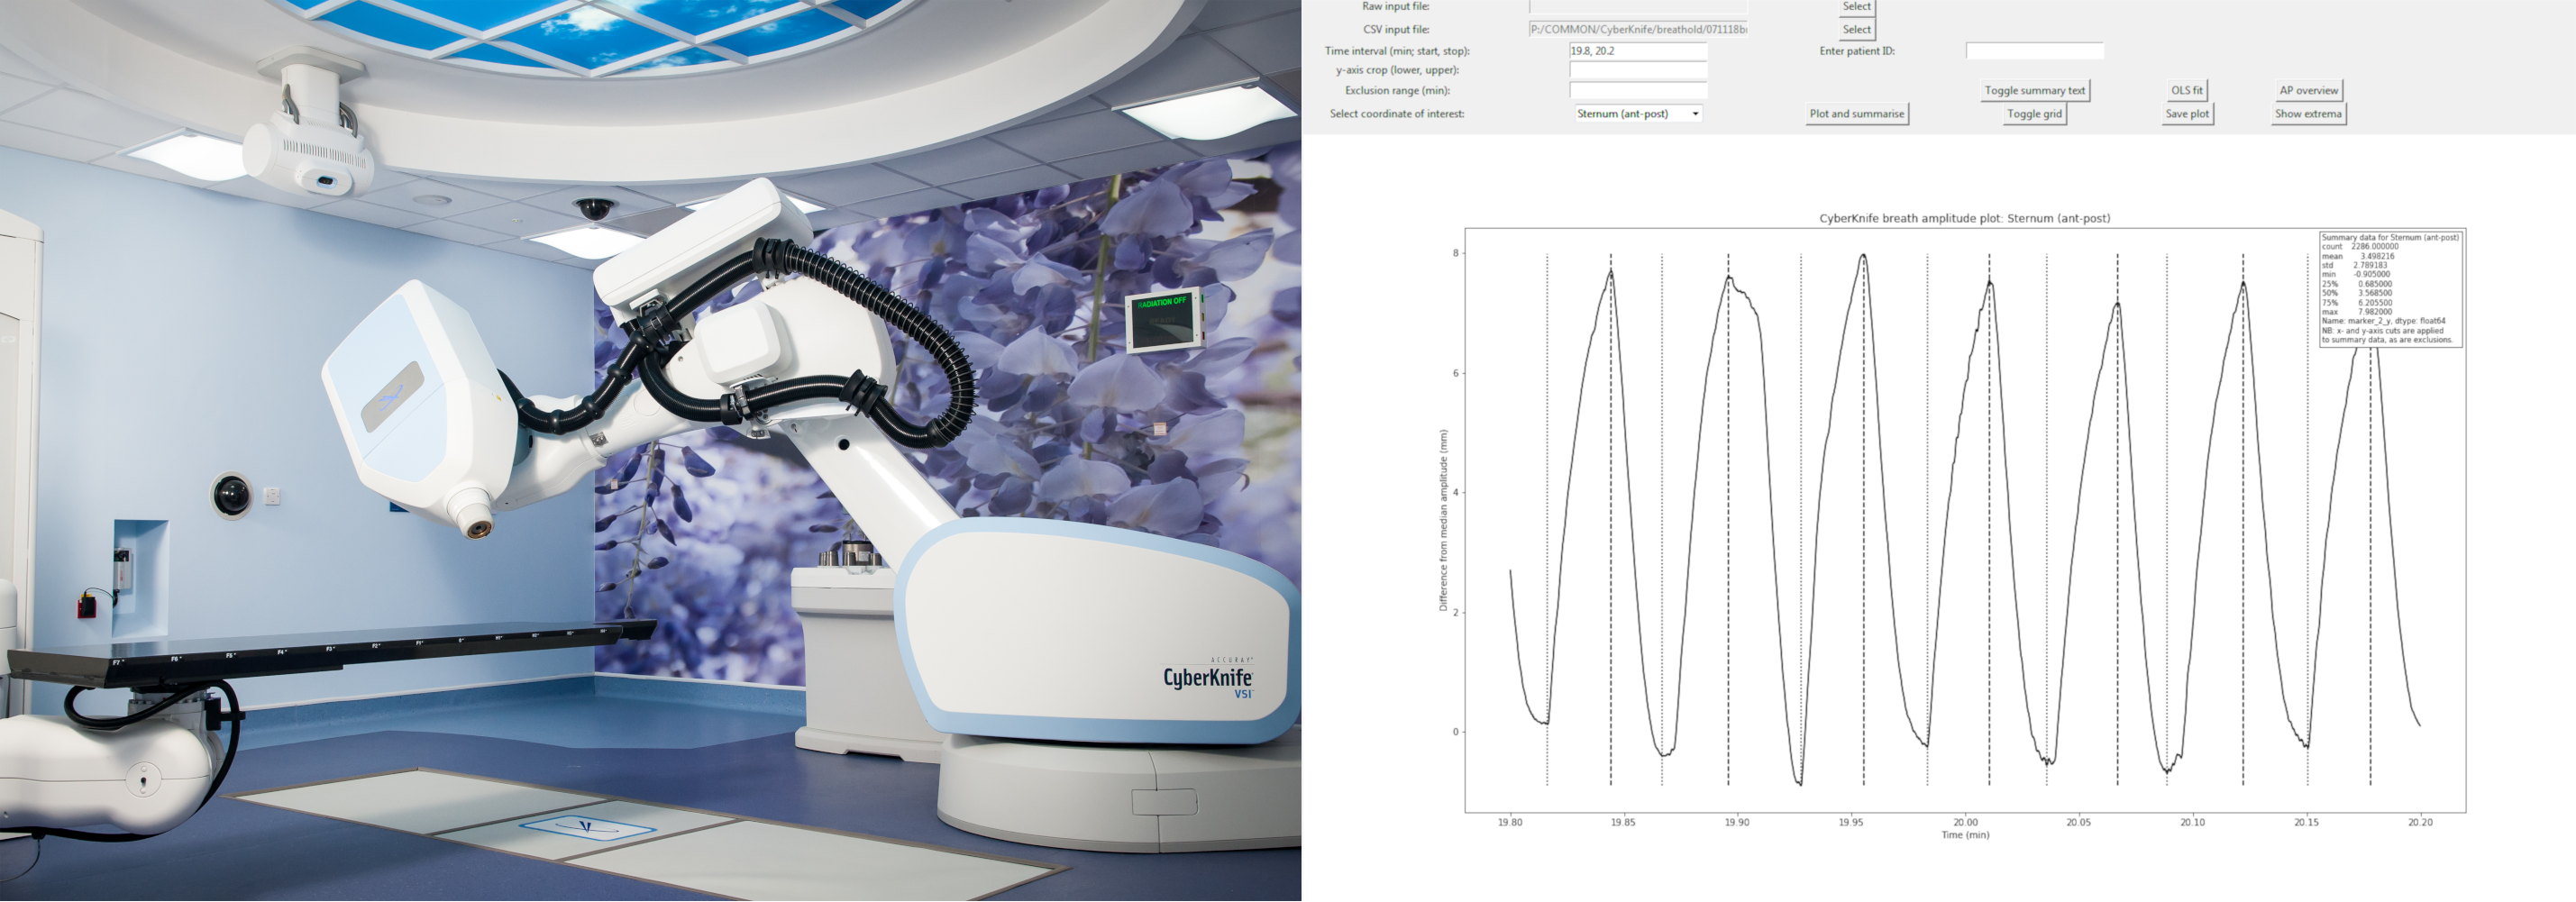
\includegraphics[width=\textwidth]{ck_with_software.png}
            \caption*{CyberKnife is a high-precision radiosurgery unit used for treatments involving several small targets. A bespoke tool (R) was developed in Python for analysis of patient breathing positional data acquired using external fiducial markers.}
        \end{figure}
    \end{block}
%
    \begin{block}{Pre-treatment image optimisation}
        \begin{figure}
            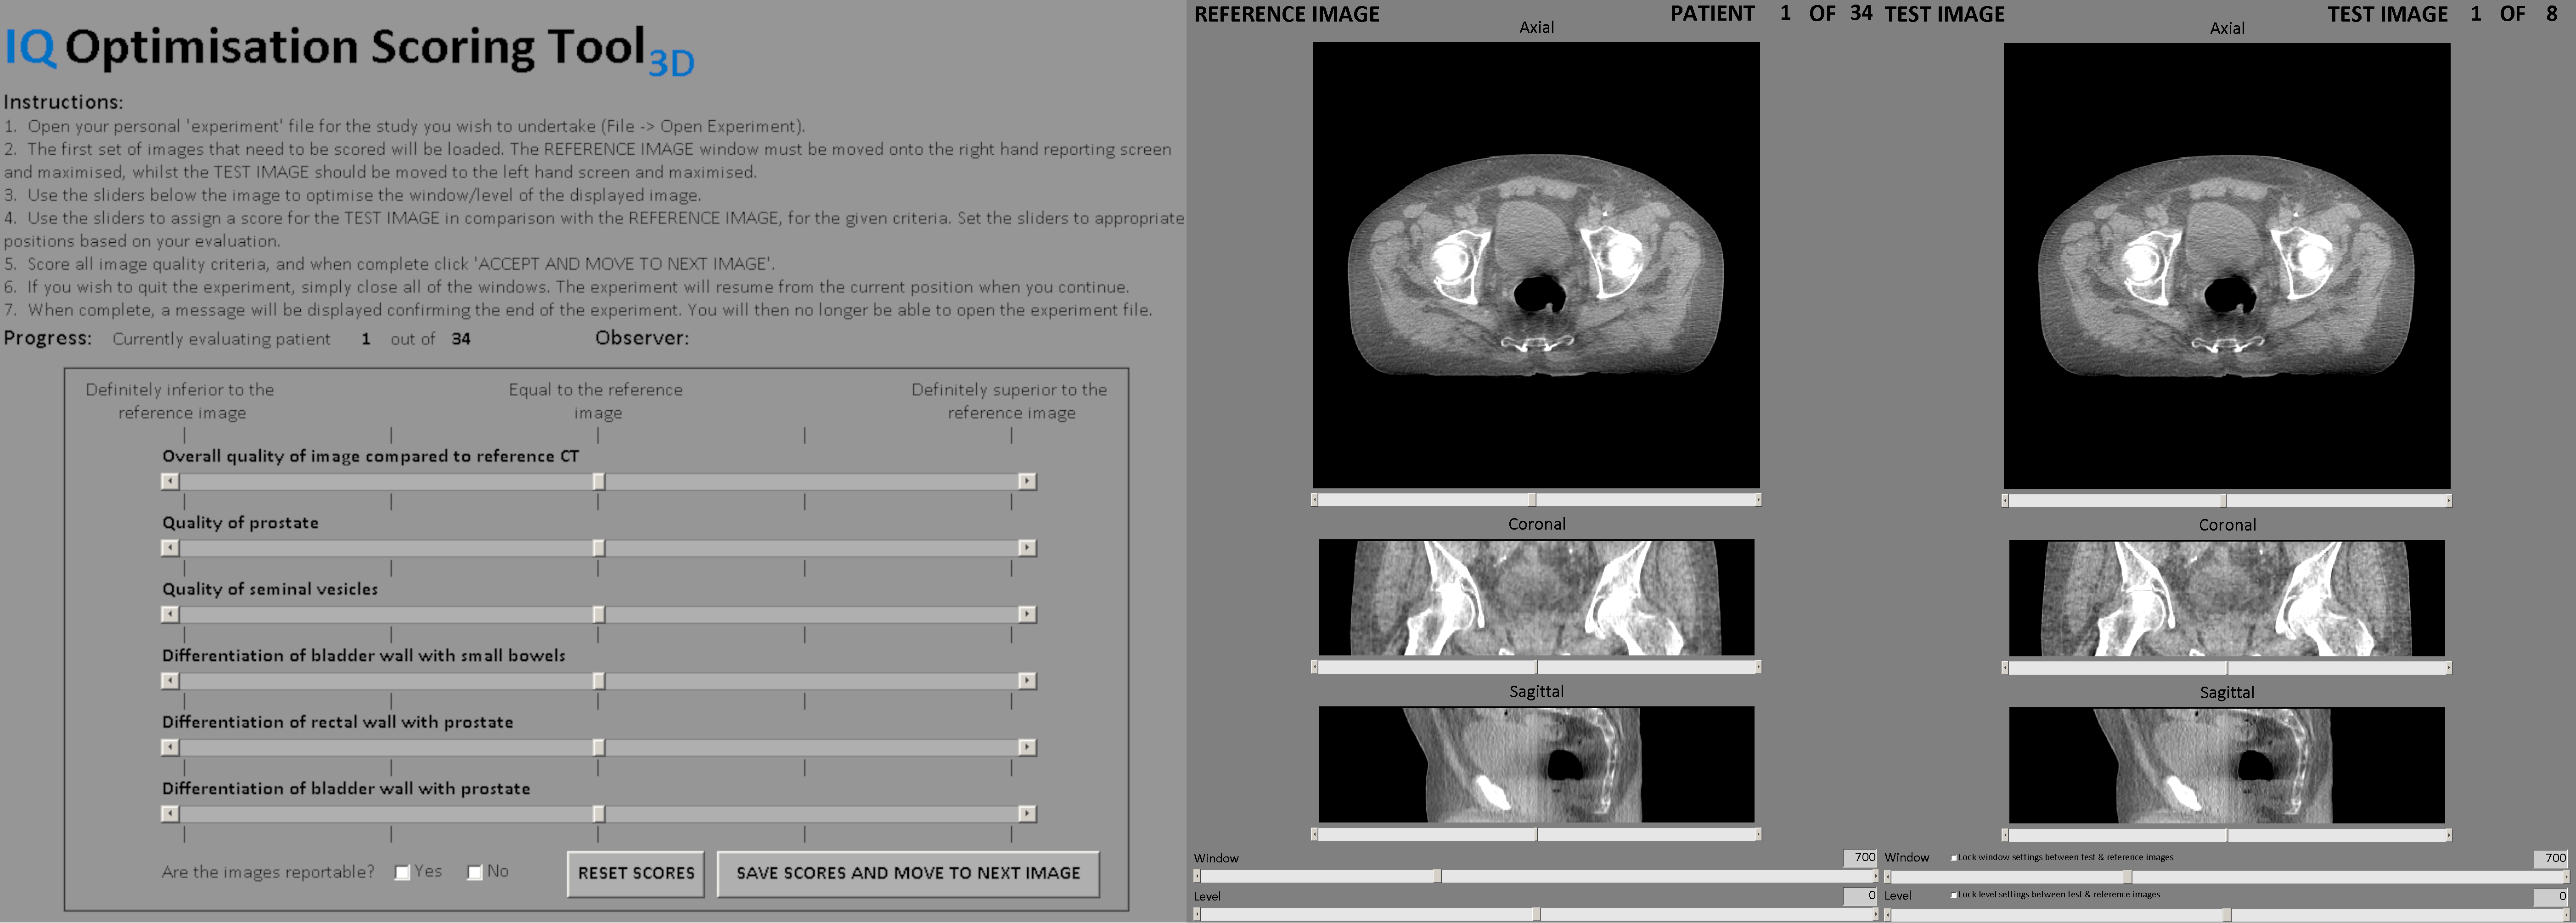
\includegraphics[width=\textwidth]{cbct_scoring_best.png}
            \caption*{The MATLAB tool used to assess the subjective image quality of reconstructed pre-treatment cone-beam CT images.}\label{fig:cbct_scoring}
        \end{figure}
        \vspace{-5 mm}
        \begin{itemize} \small
        \item Aimed to compare images reconstructed using random variations on the reconstruction parameters to those using default values.
        \item Blinded radiographers scored each test image according to a set of predefined criteria.
        \item A linear mixed-effect regression model was fit to the data in R, to quantify the effect of varying each parameter independently.
        \item Phantom measurements with a range of X-ray tube voltages and currents ${\rightarrow}$ derivation of optimal exposure factors for a range of patient weight categories.
        \end{itemize}
    \end{block}
\end{textblock}
\end{frame}
\end{document}
